% Options for packages loaded elsewhere
\PassOptionsToPackage{unicode}{hyperref}
\PassOptionsToPackage{hyphens}{url}
%
\documentclass[
  ignorenonframetext,
]{beamer}
\usepackage{pgfpages}
\setbeamertemplate{caption}[numbered]
\setbeamertemplate{caption label separator}{: }
\setbeamercolor{caption name}{fg=normal text.fg}
\beamertemplatenavigationsymbolsempty
% Prevent slide breaks in the middle of a paragraph
\widowpenalties 1 10000
\raggedbottom
\setbeamertemplate{part page}{
  \centering
  \begin{beamercolorbox}[sep=16pt,center]{part title}
    \usebeamerfont{part title}\insertpart\par
  \end{beamercolorbox}
}
\setbeamertemplate{section page}{
  \centering
  \begin{beamercolorbox}[sep=12pt,center]{part title}
    \usebeamerfont{section title}\insertsection\par
  \end{beamercolorbox}
}
\setbeamertemplate{subsection page}{
  \centering
  \begin{beamercolorbox}[sep=8pt,center]{part title}
    \usebeamerfont{subsection title}\insertsubsection\par
  \end{beamercolorbox}
}
\AtBeginPart{
  \frame{\partpage}
}
\AtBeginSection{
  \ifbibliography
  \else
    \frame{\sectionpage}
  \fi
}
\AtBeginSubsection{
  \frame{\subsectionpage}
}
\usepackage{lmodern}
\usepackage{amssymb,amsmath}
\usepackage{ifxetex,ifluatex}
\ifnum 0\ifxetex 1\fi\ifluatex 1\fi=0 % if pdftex
  \usepackage[T1]{fontenc}
  \usepackage[utf8]{inputenc}
  \usepackage{textcomp} % provide euro and other symbols
\else % if luatex or xetex
  \usepackage{unicode-math}
  \defaultfontfeatures{Scale=MatchLowercase}
  \defaultfontfeatures[\rmfamily]{Ligatures=TeX,Scale=1}
\fi
% Use upquote if available, for straight quotes in verbatim environments
\IfFileExists{upquote.sty}{\usepackage{upquote}}{}
\IfFileExists{microtype.sty}{% use microtype if available
  \usepackage[]{microtype}
  \UseMicrotypeSet[protrusion]{basicmath} % disable protrusion for tt fonts
}{}
\makeatletter
\@ifundefined{KOMAClassName}{% if non-KOMA class
  \IfFileExists{parskip.sty}{%
    \usepackage{parskip}
  }{% else
    \setlength{\parindent}{0pt}
    \setlength{\parskip}{6pt plus 2pt minus 1pt}}
}{% if KOMA class
  \KOMAoptions{parskip=half}}
\makeatother
\usepackage{xcolor}
\IfFileExists{xurl.sty}{\usepackage{xurl}}{} % add URL line breaks if available
\IfFileExists{bookmark.sty}{\usepackage{bookmark}}{\usepackage{hyperref}}
\hypersetup{
  pdftitle={Module 1: Introduction to Bayesian Statistics},
  pdfauthor={Rebecca C. Steorts},
  hidelinks,
  pdfcreator={LaTeX via pandoc}}
\urlstyle{same} % disable monospaced font for URLs
\newif\ifbibliography
\usepackage{color}
\usepackage{fancyvrb}
\newcommand{\VerbBar}{|}
\newcommand{\VERB}{\Verb[commandchars=\\\{\}]}
\DefineVerbatimEnvironment{Highlighting}{Verbatim}{commandchars=\\\{\}}
% Add ',fontsize=\small' for more characters per line
\usepackage{framed}
\definecolor{shadecolor}{RGB}{248,248,248}
\newenvironment{Shaded}{\begin{snugshade}}{\end{snugshade}}
\newcommand{\AlertTok}[1]{\textcolor[rgb]{0.94,0.16,0.16}{#1}}
\newcommand{\AnnotationTok}[1]{\textcolor[rgb]{0.56,0.35,0.01}{\textbf{\textit{#1}}}}
\newcommand{\AttributeTok}[1]{\textcolor[rgb]{0.77,0.63,0.00}{#1}}
\newcommand{\BaseNTok}[1]{\textcolor[rgb]{0.00,0.00,0.81}{#1}}
\newcommand{\BuiltInTok}[1]{#1}
\newcommand{\CharTok}[1]{\textcolor[rgb]{0.31,0.60,0.02}{#1}}
\newcommand{\CommentTok}[1]{\textcolor[rgb]{0.56,0.35,0.01}{\textit{#1}}}
\newcommand{\CommentVarTok}[1]{\textcolor[rgb]{0.56,0.35,0.01}{\textbf{\textit{#1}}}}
\newcommand{\ConstantTok}[1]{\textcolor[rgb]{0.00,0.00,0.00}{#1}}
\newcommand{\ControlFlowTok}[1]{\textcolor[rgb]{0.13,0.29,0.53}{\textbf{#1}}}
\newcommand{\DataTypeTok}[1]{\textcolor[rgb]{0.13,0.29,0.53}{#1}}
\newcommand{\DecValTok}[1]{\textcolor[rgb]{0.00,0.00,0.81}{#1}}
\newcommand{\DocumentationTok}[1]{\textcolor[rgb]{0.56,0.35,0.01}{\textbf{\textit{#1}}}}
\newcommand{\ErrorTok}[1]{\textcolor[rgb]{0.64,0.00,0.00}{\textbf{#1}}}
\newcommand{\ExtensionTok}[1]{#1}
\newcommand{\FloatTok}[1]{\textcolor[rgb]{0.00,0.00,0.81}{#1}}
\newcommand{\FunctionTok}[1]{\textcolor[rgb]{0.00,0.00,0.00}{#1}}
\newcommand{\ImportTok}[1]{#1}
\newcommand{\InformationTok}[1]{\textcolor[rgb]{0.56,0.35,0.01}{\textbf{\textit{#1}}}}
\newcommand{\KeywordTok}[1]{\textcolor[rgb]{0.13,0.29,0.53}{\textbf{#1}}}
\newcommand{\NormalTok}[1]{#1}
\newcommand{\OperatorTok}[1]{\textcolor[rgb]{0.81,0.36,0.00}{\textbf{#1}}}
\newcommand{\OtherTok}[1]{\textcolor[rgb]{0.56,0.35,0.01}{#1}}
\newcommand{\PreprocessorTok}[1]{\textcolor[rgb]{0.56,0.35,0.01}{\textit{#1}}}
\newcommand{\RegionMarkerTok}[1]{#1}
\newcommand{\SpecialCharTok}[1]{\textcolor[rgb]{0.00,0.00,0.00}{#1}}
\newcommand{\SpecialStringTok}[1]{\textcolor[rgb]{0.31,0.60,0.02}{#1}}
\newcommand{\StringTok}[1]{\textcolor[rgb]{0.31,0.60,0.02}{#1}}
\newcommand{\VariableTok}[1]{\textcolor[rgb]{0.00,0.00,0.00}{#1}}
\newcommand{\VerbatimStringTok}[1]{\textcolor[rgb]{0.31,0.60,0.02}{#1}}
\newcommand{\WarningTok}[1]{\textcolor[rgb]{0.56,0.35,0.01}{\textbf{\textit{#1}}}}
\usepackage{graphicx,grffile}
\makeatletter
\def\maxwidth{\ifdim\Gin@nat@width>\linewidth\linewidth\else\Gin@nat@width\fi}
\def\maxheight{\ifdim\Gin@nat@height>\textheight\textheight\else\Gin@nat@height\fi}
\makeatother
% Scale images if necessary, so that they will not overflow the page
% margins by default, and it is still possible to overwrite the defaults
% using explicit options in \includegraphics[width, height, ...]{}
\setkeys{Gin}{width=\maxwidth,height=\maxheight,keepaspectratio}
% Set default figure placement to htbp
\makeatletter
\def\fps@figure{htbp}
\makeatother
\setlength{\emergencystretch}{3em} % prevent overfull lines
\providecommand{\tightlist}{%
  \setlength{\itemsep}{0pt}\setlength{\parskip}{0pt}}
\setcounter{secnumdepth}{-\maxdimen} % remove section numbering
% Custom definitions
% To use this customization file, insert the line "% Custom definitions
% To use this customization file, insert the line "% Custom definitions
% To use this customization file, insert the line "% Custom definitions
% To use this customization file, insert the line "\input{custom}" in the header of the tex file.

% Formatting

\tolerance=1000
\usepackage[margin=1in]{geometry}


% Packages

% \usepackage{amssymb,latexsym}
\usepackage{amssymb,amsfonts,amsmath,latexsym,amsthm}
\usepackage[usenames,dvipsnames]{color}
\usepackage[]{graphicx}
\usepackage[space]{grffile}
\usepackage{mathrsfs}   % fancy math font
% \usepackage[font=small,skip=0pt]{caption}
\usepackage[skip=0pt]{caption}
\usepackage{subcaption}
\usepackage{verbatim}
\usepackage{url}
\usepackage{bm}
\usepackage{dsfont}
\usepackage{extarrows}
\usepackage{multirow}
% \usepackage{wrapfig}
% \usepackage{epstopdf}
\usepackage{rotating}
\usepackage{tikz}
\usetikzlibrary{fit}					% fitting shapes to coordinates
%\usetikzlibrary{backgrounds}	% drawing the background after the foreground


% \usepackage[dvipdfm,colorlinks,citecolor=blue,linkcolor=blue,urlcolor=blue]{hyperref}
\usepackage[colorlinks,citecolor=blue,linkcolor=blue,urlcolor=blue]{hyperref}
%\usepackage{hyperref}
\usepackage[authoryear,round]{natbib}


%  Theorems, etc.

\theoremstyle{plain}
\newtheorem{theorem}{Theorem}[section]
\newtheorem{corollary}[theorem]{Corollary}
\newtheorem{lemma}[theorem]{Lemma}
\newtheorem{proposition}[theorem]{Proposition}
\newtheorem{condition}[theorem]{Condition}
% \newtheorem{conditions}[theorem]{Conditions}

\theoremstyle{definition}
\newtheorem{definition}[theorem]{Definition}
% \newtheorem*{unnumbered-definition}{Definition}
\newtheorem{example}[theorem]{Example}
\theoremstyle{remark}
\newtheorem*{remark}{Remark}
\numberwithin{equation}{section}




% Document-specific shortcuts
\newcommand{\btheta}{{\bm\theta}}
\newcommand{\bbtheta}{{\pmb{\bm\theta}}}

\newcommand{\commentary}[1]{\ifx\showcommentary\undefined\else \emph{#1}\fi}

\newcommand{\term}[1]{\textit{\textbf{#1}}}

% Math shortcuts

% Probability distributions
\DeclareMathOperator*{\Exp}{Exp}
\DeclareMathOperator*{\TExp}{TExp}
\DeclareMathOperator*{\Bernoulli}{Bernoulli}
\DeclareMathOperator*{\Beta}{Beta}
\DeclareMathOperator*{\Ga}{Gamma}
\DeclareMathOperator*{\TGamma}{TGamma}
\DeclareMathOperator*{\Poisson}{Poisson}
\DeclareMathOperator*{\Binomial}{Binomial}
\DeclareMathOperator*{\NormalGamma}{NormalGamma}
\DeclareMathOperator*{\InvGamma}{InvGamma}
\DeclareMathOperator*{\Cauchy}{Cauchy}
\DeclareMathOperator*{\Uniform}{Uniform}
\DeclareMathOperator*{\Gumbel}{Gumbel}
\DeclareMathOperator*{\Pareto}{Pareto}
\DeclareMathOperator*{\Mono}{Mono}
\DeclareMathOperator*{\Geometric}{Geometric}
\DeclareMathOperator*{\Wishart}{Wishart}

% Math operators
\DeclareMathOperator*{\argmin}{arg\,min}
\DeclareMathOperator*{\argmax}{arg\,max}
\DeclareMathOperator*{\Cov}{Cov}
\DeclareMathOperator*{\diag}{diag}
\DeclareMathOperator*{\median}{median}
\DeclareMathOperator*{\Vol}{Vol}

% Math characters
\newcommand{\R}{\mathbb{R}}
\newcommand{\Z}{\mathbb{Z}}
\newcommand{\E}{\mathbb{E}}
\renewcommand{\Pr}{\mathbb{P}}
\newcommand{\I}{\mathds{1}}
\newcommand{\V}{\mathbb{V}}

\newcommand{\A}{\mathcal{A}}
\newcommand{\C}{\mathcal{C}}
\newcommand{\D}{\mathcal{D}}
\newcommand{\Hcal}{\mathcal{H}}
\newcommand{\M}{\mathcal{M}}
\newcommand{\N}{\mathcal{N}}
\newcommand{\X}{\mathcal{X}}
\newcommand{\Zcal}{\mathcal{Z}}
\renewcommand{\P}{\mathcal{P}}

\newcommand{\T}{\mathtt{T}}
\renewcommand{\emptyset}{\varnothing}


% Miscellaneous commands
\newcommand{\iid}{\stackrel{\mathrm{iid}}{\sim}}
\newcommand{\matrixsmall}[1]{\bigl(\begin{smallmatrix}#1\end{smallmatrix} \bigr)}

\newcommand{\items}[1]{\begin{itemize} #1 \end{itemize}}

\newcommand{\todo}[1]{\emph{\textcolor{red}{(#1)}}}

\newcommand{\branch}[4]{
\left\{
	\begin{array}{ll}
		#1  & \mbox{if } #2 \\
		#3 & \mbox{if } #4
	\end{array}
\right.
}

% approximately proportional to
\def\app#1#2{%
  \mathrel{%
    \setbox0=\hbox{$#1\sim$}%
    \setbox2=\hbox{%
      \rlap{\hbox{$#1\propto$}}%
      \lower1.3\ht0\box0%
    }%
    \raise0.25\ht2\box2%
  }%
}
\def\approxprop{\mathpalette\app\relax}

% \newcommand{\approptoinn}[2]{\mathrel{\vcenter{
  % \offinterlineskip\halign{\hfil$##$\cr
    % #1\propto\cr\noalign{\kern2pt}#1\sim\cr\noalign{\kern-2pt}}}}}

% \newcommand{\approxpropto}{\mathpalette\approptoinn\relax}





" in the header of the tex file.

% Formatting

\tolerance=1000
\usepackage[margin=1in]{geometry}


% Packages

% \usepackage{amssymb,latexsym}
\usepackage{amssymb,amsfonts,amsmath,latexsym,amsthm}
\usepackage[usenames,dvipsnames]{color}
\usepackage[]{graphicx}
\usepackage[space]{grffile}
\usepackage{mathrsfs}   % fancy math font
% \usepackage[font=small,skip=0pt]{caption}
\usepackage[skip=0pt]{caption}
\usepackage{subcaption}
\usepackage{verbatim}
\usepackage{url}
\usepackage{bm}
\usepackage{dsfont}
\usepackage{extarrows}
\usepackage{multirow}
% \usepackage{wrapfig}
% \usepackage{epstopdf}
\usepackage{rotating}
\usepackage{tikz}
\usetikzlibrary{fit}					% fitting shapes to coordinates
%\usetikzlibrary{backgrounds}	% drawing the background after the foreground


% \usepackage[dvipdfm,colorlinks,citecolor=blue,linkcolor=blue,urlcolor=blue]{hyperref}
\usepackage[colorlinks,citecolor=blue,linkcolor=blue,urlcolor=blue]{hyperref}
%\usepackage{hyperref}
\usepackage[authoryear,round]{natbib}


%  Theorems, etc.

\theoremstyle{plain}
\newtheorem{theorem}{Theorem}[section]
\newtheorem{corollary}[theorem]{Corollary}
\newtheorem{lemma}[theorem]{Lemma}
\newtheorem{proposition}[theorem]{Proposition}
\newtheorem{condition}[theorem]{Condition}
% \newtheorem{conditions}[theorem]{Conditions}

\theoremstyle{definition}
\newtheorem{definition}[theorem]{Definition}
% \newtheorem*{unnumbered-definition}{Definition}
\newtheorem{example}[theorem]{Example}
\theoremstyle{remark}
\newtheorem*{remark}{Remark}
\numberwithin{equation}{section}




% Document-specific shortcuts
\newcommand{\btheta}{{\bm\theta}}
\newcommand{\bbtheta}{{\pmb{\bm\theta}}}

\newcommand{\commentary}[1]{\ifx\showcommentary\undefined\else \emph{#1}\fi}

\newcommand{\term}[1]{\textit{\textbf{#1}}}

% Math shortcuts

% Probability distributions
\DeclareMathOperator*{\Exp}{Exp}
\DeclareMathOperator*{\TExp}{TExp}
\DeclareMathOperator*{\Bernoulli}{Bernoulli}
\DeclareMathOperator*{\Beta}{Beta}
\DeclareMathOperator*{\Ga}{Gamma}
\DeclareMathOperator*{\TGamma}{TGamma}
\DeclareMathOperator*{\Poisson}{Poisson}
\DeclareMathOperator*{\Binomial}{Binomial}
\DeclareMathOperator*{\NormalGamma}{NormalGamma}
\DeclareMathOperator*{\InvGamma}{InvGamma}
\DeclareMathOperator*{\Cauchy}{Cauchy}
\DeclareMathOperator*{\Uniform}{Uniform}
\DeclareMathOperator*{\Gumbel}{Gumbel}
\DeclareMathOperator*{\Pareto}{Pareto}
\DeclareMathOperator*{\Mono}{Mono}
\DeclareMathOperator*{\Geometric}{Geometric}
\DeclareMathOperator*{\Wishart}{Wishart}

% Math operators
\DeclareMathOperator*{\argmin}{arg\,min}
\DeclareMathOperator*{\argmax}{arg\,max}
\DeclareMathOperator*{\Cov}{Cov}
\DeclareMathOperator*{\diag}{diag}
\DeclareMathOperator*{\median}{median}
\DeclareMathOperator*{\Vol}{Vol}

% Math characters
\newcommand{\R}{\mathbb{R}}
\newcommand{\Z}{\mathbb{Z}}
\newcommand{\E}{\mathbb{E}}
\renewcommand{\Pr}{\mathbb{P}}
\newcommand{\I}{\mathds{1}}
\newcommand{\V}{\mathbb{V}}

\newcommand{\A}{\mathcal{A}}
\newcommand{\C}{\mathcal{C}}
\newcommand{\D}{\mathcal{D}}
\newcommand{\Hcal}{\mathcal{H}}
\newcommand{\M}{\mathcal{M}}
\newcommand{\N}{\mathcal{N}}
\newcommand{\X}{\mathcal{X}}
\newcommand{\Zcal}{\mathcal{Z}}
\renewcommand{\P}{\mathcal{P}}

\newcommand{\T}{\mathtt{T}}
\renewcommand{\emptyset}{\varnothing}


% Miscellaneous commands
\newcommand{\iid}{\stackrel{\mathrm{iid}}{\sim}}
\newcommand{\matrixsmall}[1]{\bigl(\begin{smallmatrix}#1\end{smallmatrix} \bigr)}

\newcommand{\items}[1]{\begin{itemize} #1 \end{itemize}}

\newcommand{\todo}[1]{\emph{\textcolor{red}{(#1)}}}

\newcommand{\branch}[4]{
\left\{
	\begin{array}{ll}
		#1  & \mbox{if } #2 \\
		#3 & \mbox{if } #4
	\end{array}
\right.
}

% approximately proportional to
\def\app#1#2{%
  \mathrel{%
    \setbox0=\hbox{$#1\sim$}%
    \setbox2=\hbox{%
      \rlap{\hbox{$#1\propto$}}%
      \lower1.3\ht0\box0%
    }%
    \raise0.25\ht2\box2%
  }%
}
\def\approxprop{\mathpalette\app\relax}

% \newcommand{\approptoinn}[2]{\mathrel{\vcenter{
  % \offinterlineskip\halign{\hfil$##$\cr
    % #1\propto\cr\noalign{\kern2pt}#1\sim\cr\noalign{\kern-2pt}}}}}

% \newcommand{\approxpropto}{\mathpalette\approptoinn\relax}





" in the header of the tex file.

% Formatting

\tolerance=1000
\usepackage[margin=1in]{geometry}


% Packages

% \usepackage{amssymb,latexsym}
\usepackage{amssymb,amsfonts,amsmath,latexsym,amsthm}
\usepackage[usenames,dvipsnames]{color}
\usepackage[]{graphicx}
\usepackage[space]{grffile}
\usepackage{mathrsfs}   % fancy math font
% \usepackage[font=small,skip=0pt]{caption}
\usepackage[skip=0pt]{caption}
\usepackage{subcaption}
\usepackage{verbatim}
\usepackage{url}
\usepackage{bm}
\usepackage{dsfont}
\usepackage{extarrows}
\usepackage{multirow}
% \usepackage{wrapfig}
% \usepackage{epstopdf}
\usepackage{rotating}
\usepackage{tikz}
\usetikzlibrary{fit}					% fitting shapes to coordinates
%\usetikzlibrary{backgrounds}	% drawing the background after the foreground


% \usepackage[dvipdfm,colorlinks,citecolor=blue,linkcolor=blue,urlcolor=blue]{hyperref}
\usepackage[colorlinks,citecolor=blue,linkcolor=blue,urlcolor=blue]{hyperref}
%\usepackage{hyperref}
\usepackage[authoryear,round]{natbib}


%  Theorems, etc.

\theoremstyle{plain}
\newtheorem{theorem}{Theorem}[section]
\newtheorem{corollary}[theorem]{Corollary}
\newtheorem{lemma}[theorem]{Lemma}
\newtheorem{proposition}[theorem]{Proposition}
\newtheorem{condition}[theorem]{Condition}
% \newtheorem{conditions}[theorem]{Conditions}

\theoremstyle{definition}
\newtheorem{definition}[theorem]{Definition}
% \newtheorem*{unnumbered-definition}{Definition}
\newtheorem{example}[theorem]{Example}
\theoremstyle{remark}
\newtheorem*{remark}{Remark}
\numberwithin{equation}{section}




% Document-specific shortcuts
\newcommand{\btheta}{{\bm\theta}}
\newcommand{\bbtheta}{{\pmb{\bm\theta}}}

\newcommand{\commentary}[1]{\ifx\showcommentary\undefined\else \emph{#1}\fi}

\newcommand{\term}[1]{\textit{\textbf{#1}}}

% Math shortcuts

% Probability distributions
\DeclareMathOperator*{\Exp}{Exp}
\DeclareMathOperator*{\TExp}{TExp}
\DeclareMathOperator*{\Bernoulli}{Bernoulli}
\DeclareMathOperator*{\Beta}{Beta}
\DeclareMathOperator*{\Ga}{Gamma}
\DeclareMathOperator*{\TGamma}{TGamma}
\DeclareMathOperator*{\Poisson}{Poisson}
\DeclareMathOperator*{\Binomial}{Binomial}
\DeclareMathOperator*{\NormalGamma}{NormalGamma}
\DeclareMathOperator*{\InvGamma}{InvGamma}
\DeclareMathOperator*{\Cauchy}{Cauchy}
\DeclareMathOperator*{\Uniform}{Uniform}
\DeclareMathOperator*{\Gumbel}{Gumbel}
\DeclareMathOperator*{\Pareto}{Pareto}
\DeclareMathOperator*{\Mono}{Mono}
\DeclareMathOperator*{\Geometric}{Geometric}
\DeclareMathOperator*{\Wishart}{Wishart}

% Math operators
\DeclareMathOperator*{\argmin}{arg\,min}
\DeclareMathOperator*{\argmax}{arg\,max}
\DeclareMathOperator*{\Cov}{Cov}
\DeclareMathOperator*{\diag}{diag}
\DeclareMathOperator*{\median}{median}
\DeclareMathOperator*{\Vol}{Vol}

% Math characters
\newcommand{\R}{\mathbb{R}}
\newcommand{\Z}{\mathbb{Z}}
\newcommand{\E}{\mathbb{E}}
\renewcommand{\Pr}{\mathbb{P}}
\newcommand{\I}{\mathds{1}}
\newcommand{\V}{\mathbb{V}}

\newcommand{\A}{\mathcal{A}}
\newcommand{\C}{\mathcal{C}}
\newcommand{\D}{\mathcal{D}}
\newcommand{\Hcal}{\mathcal{H}}
\newcommand{\M}{\mathcal{M}}
\newcommand{\N}{\mathcal{N}}
\newcommand{\X}{\mathcal{X}}
\newcommand{\Zcal}{\mathcal{Z}}
\renewcommand{\P}{\mathcal{P}}

\newcommand{\T}{\mathtt{T}}
\renewcommand{\emptyset}{\varnothing}


% Miscellaneous commands
\newcommand{\iid}{\stackrel{\mathrm{iid}}{\sim}}
\newcommand{\matrixsmall}[1]{\bigl(\begin{smallmatrix}#1\end{smallmatrix} \bigr)}

\newcommand{\items}[1]{\begin{itemize} #1 \end{itemize}}

\newcommand{\todo}[1]{\emph{\textcolor{red}{(#1)}}}

\newcommand{\branch}[4]{
\left\{
	\begin{array}{ll}
		#1  & \mbox{if } #2 \\
		#3 & \mbox{if } #4
	\end{array}
\right.
}

% approximately proportional to
\def\app#1#2{%
  \mathrel{%
    \setbox0=\hbox{$#1\sim$}%
    \setbox2=\hbox{%
      \rlap{\hbox{$#1\propto$}}%
      \lower1.3\ht0\box0%
    }%
    \raise0.25\ht2\box2%
  }%
}
\def\approxprop{\mathpalette\app\relax}

% \newcommand{\approptoinn}[2]{\mathrel{\vcenter{
  % \offinterlineskip\halign{\hfil$##$\cr
    % #1\propto\cr\noalign{\kern2pt}#1\sim\cr\noalign{\kern-2pt}}}}}

% \newcommand{\approxpropto}{\mathpalette\approptoinn\relax}





" in the header of the tex file.

% Formatting




% Packages

\setbeamertemplate{navigation symbols}{}
\setbeamertemplate{footline}[page number]

 \usepackage{amssymb,latexsym}
\usepackage{amssymb,amsfonts,amsmath,latexsym,amsthm, bm}
%\usepackage[usenames,dvipsnames]{color}
%\usepackage[]{graphicx}
%\usepackage[space]{grffile}
\usepackage{mathrsfs}   % fancy math font
% \usepackage[font=small,skip=0pt]{caption}
%\usepackage[skip=0pt]{caption}
%\usepackage{subcaption}
%\usepackage{verbatim}
%\usepackage{url}
%\usepackage{bm}
\usepackage{dsfont}
\usepackage{multirow}
%\usepackage{extarrows}
%\usepackage{multirow}
%% \usepackage{wrapfig}
%% \usepackage{epstopdf}
%\usepackage{rotating}
%\usepackage{tikz}
%\usetikzlibrary{fit}					% fitting shapes to coordinates
%\usetikzlibrary{backgrounds}	% drawing the background after the foreground


% \usepackage[dvipdfm,colorlinks,citecolor=blue,linkcolor=blue,urlcolor=blue]{hyperref}
%\usepackage[colorlinks,citecolor=blue,linkcolor=blue,urlcolor=blue]{hyperref}
%%\usepackage{hyperref}
%\usepackage[authoryear,round]{natbib}


%  Theorems, etc.

%\theoremstyle{plain}
%\newtheorem{theorem}{Theorem}[section]
%\newtheorem{corollary}[theorem]{Corollary}
%\newtheorem{lemma}[theorem]{Lemma}
%\newtheorem{proposition}[theorem]{Proposition}
%\newtheorem{condition}[theorem]{Condition}
% \newtheorem{conditions}[theorem]{Conditions}

%\theoremstyle{definition}
%\newtheorem{definition}[theorem]{Definition}
%% \newtheorem*{unnumbered-definition}{Definition}
%\newtheorem{example}[theorem]{Example}
%\theoremstyle{remark}
%\newtheorem*{remark}{Remark}
%\numberwithin{equation}{section}




% Document-specific shortcuts
\newcommand{\btheta}{{\bm\theta}}
\newcommand{\bbtheta}{{\pmb{\bm\theta}}}

\newcommand{\commentary}[1]{\ifx\showcommentary\undefined\else \emph{#1}\fi}

\newcommand{\term}[1]{\textit{\textbf{#1}}}

% Math shortcuts

% Probability distributions
\DeclareMathOperator*{\Exp}{Exp}
\DeclareMathOperator*{\TExp}{TExp}
\DeclareMathOperator*{\Bernoulli}{Bernoulli}
\DeclareMathOperator*{\Beta}{Beta}
\DeclareMathOperator*{\Ga}{Gamma}
\DeclareMathOperator*{\TGamma}{TGamma}
\DeclareMathOperator*{\Poisson}{Poisson}
\DeclareMathOperator*{\Binomial}{Binomial}
\DeclareMathOperator*{\NormalGamma}{NormalGamma}
\DeclareMathOperator*{\InvGamma}{InvGamma}
\DeclareMathOperator*{\Cauchy}{Cauchy}
\DeclareMathOperator*{\Uniform}{Uniform}
\DeclareMathOperator*{\Gumbel}{Gumbel}
\DeclareMathOperator*{\Pareto}{Pareto}
\DeclareMathOperator*{\Mono}{Mono}
\DeclareMathOperator*{\Geometric}{Geometric}
\DeclareMathOperator*{\Wishart}{Wishart}

% Math operators
\DeclareMathOperator*{\argmin}{arg\,min}
\DeclareMathOperator*{\argmax}{arg\,max}
\DeclareMathOperator*{\Cov}{Cov}
\DeclareMathOperator*{\diag}{diag}
\DeclareMathOperator*{\median}{median}
\DeclareMathOperator*{\Vol}{Vol}

% Math characters
\newcommand{\R}{\mathbb{R}}
\newcommand{\Z}{\mathbb{Z}}
\newcommand{\E}{\mathbb{E}}
\renewcommand{\Pr}{\mathbb{P}}
\newcommand{\I}{\mathds{1}}
\newcommand{\V}{\mathbb{V}}

\newcommand{\A}{\mathcal{A}}
%\newcommand{\C}{\mathcal{C}}
\newcommand{\D}{\mathcal{D}}
\newcommand{\Hcal}{\mathcal{H}}
\newcommand{\M}{\mathcal{M}}
\newcommand{\N}{\mathcal{N}}
\newcommand{\X}{\mathcal{X}}
\newcommand{\Zcal}{\mathcal{Z}}
\renewcommand{\P}{\mathcal{P}}

\newcommand{\T}{\mathtt{T}}
\renewcommand{\emptyset}{\varnothing}


% Miscellaneous commands
\newcommand{\iid}{\stackrel{\mathrm{iid}}{\sim}}
\newcommand{\matrixsmall}[1]{\bigl(\begin{smallmatrix}#1\end{smallmatrix} \bigr)}

\newcommand{\items}[1]{\begin{itemize} #1 \end{itemize}}

\newcommand{\todo}[1]{\emph{\textcolor{red}{(#1)}}}

\newcommand{\branch}[4]{
\left\{
	\begin{array}{ll}
		#1  & \mbox{if } #2 \\
		#3 & \mbox{if } #4
	\end{array}
\right.
}

% approximately proportional to
\def\app#1#2{%
  \mathrel{%
    \setbox0=\hbox{$#1\sim$}%
    \setbox2=\hbox{%
      \rlap{\hbox{$#1\propto$}}%
      \lower1.3\ht0\box0%
    }%
    \raise0.25\ht2\box2%
  }%
}
\def\approxprop{\mathpalette\app\relax}

% \newcommand{\approptoinn}[2]{\mathrel{\vcenter{
  % \offinterlineskip\halign{\hfil$##$\cr
    % #1\propto\cr\noalign{\kern2pt}#1\sim\cr\noalign{\kern-2pt}}}}}

% \newcommand{\approxpropto}{\mathpalette\approptoinn\relax}

\title{Module 1: Introduction to Bayesian Statistics}
\author{Rebecca C. Steorts}
\date{}

\begin{document}
\frame{\titlepage}

\begin{frame}{Agenda}
\protect\hypertarget{agenda}{}

\begin{itemize}
\tightlist
\item
  Motivations
\item
  Traditional inference
\item
  Bayesian inference
\item
  Bernoulli, Beta
\item
  Posterior of Bernoulli-Beta
\item
  Conjugacy
\item
  Example with 2012 election data
\item
  No sleep example
\item
  Marginal likelihood
\item
  Posterior Prediction
\end{itemize}

\end{frame}

\begin{frame}{Traditional inference}
\protect\hypertarget{traditional-inference}{}

You are given \textbf{data} \(X\) and there is an \textbf{unknown
parameter} you wish to estimate \textbf{\(\theta\)}

How would you estimate \(\theta\)?

\begin{itemize}
\tightlist
\item
  Find an unbiased estimator of \(\theta\).
\item
  Find the maximum likelihood estimate (MLE) of \(\theta\) by looking at
  the likelihood of the data.
\item
  If you cannot remember the definition of an unbiased estimator or the
  MLE, review these before our next class.
\end{itemize}

\end{frame}

\begin{frame}{Bayesian inference}
\protect\hypertarget{bayesian-inference}{}

Bayesian methods trace its origin to the 18th century and English
Reverend Thomas Bayes, who along with Pierre-Simon Laplace discovered
what we now call \textbf{Bayes' Theorem}

\begin{itemize}
\tightlist
\item
  \(p(x \mid \theta)\) likelihood
\item
  \(p(\theta)\) prior
\item
  \(p(\theta \mid x)\) posterior
\item
  \(p(x)\) marginal distribution
\end{itemize}

Derive the posterior distribution of \(p(\theta \mid x).\)

\end{frame}

\begin{frame}{Bernoulli distribution}
\protect\hypertarget{bernoulli-distribution}{}

The Bernoulli distribution is very common due to binary outcomes.

\begin{itemize}
\tightlist
\item
  Consider flipping a coin (heads or tails).
\item
  We can represent this a binary random variable where the probability
  of heads is \(\theta\) and the probability of tails is \(1-\theta.\)
\end{itemize}

The write the random variable as
\(X \sim \Bernoulli(\theta) \I(0 < \theta < 1)\)

It follows that the likelihood is
\[p(x \mid \theta) = \theta^x (1-\theta)^{(1-x)}\I(0 < \theta < 1).\]

\begin{itemize}
\tightlist
\item
  Exercise: what is the mean and the variance of \(X\)?
\end{itemize}

\end{frame}

\begin{frame}{Bernoulli distribution}
\protect\hypertarget{bernoulli-distribution-1}{}

\begin{itemize}
\tightlist
\item
  Suppose that
  \(X_1,\ldots,X_n \stackrel{iid}{\sim} \Bernoulli(\theta).\) Then for
  \(x_1,\ldots,x_n \in \{0,1\}\) what is the likelihood?
\end{itemize}

\end{frame}

\begin{frame}{Notation}
\protect\hypertarget{notation}{}

\begin{itemize}
\tightlist
\item
  \(\propto\): means ``proportional to''
\item
  \(x_{1:n}\) denotes \(x_1,\ldots,x_n\)
\end{itemize}

\end{frame}

\begin{frame}{Likelihood}
\protect\hypertarget{likelihood}{}

\[
\begin{aligned}
p(x_{1:n}|\theta) &= \Pr(X_1 = x_1,\dotsc,X_n = x_n\mid\theta) \notag\\
& =\prod_{i = 1}^n \Pr(X_i = x_i\mid\theta) \notag\\
& = \prod_{i = 1}^n p(x_i|\theta) \notag\\
& =\prod_{i = 1}^n \theta^{x_i}(1-\theta)^{1-x_i} \notag\\
& =\theta^{\sum x_i}(1-\theta)^{n-\sum x_i}. \label{equation:likelihood}
\end{aligned}
\]

\end{frame}

\begin{frame}{Beta distribution}
\protect\hypertarget{beta-distribution}{}

Given \(a,b>0\), we write \(\theta \sim \Beta(a,b)\) to mean that
\(\theta\) has pdf

\[
p(\theta) =\Beta(\theta|a,b) =\frac{1}{B(a,b)}\theta^{a-1}(1-\theta)^{b-1}\I(0<\theta<1),
\]

i.e., \(p(\theta)\propto \theta^{a-1}(1-\theta)^{b-1}\) on the interval
from \(0\) to \(1\).

\begin{itemize}
\tightlist
\item
  Here, \[B(a,b) = \frac{\Gamma(a)\Gamma(b)}{\Gamma(a+b)}\].
\item
  The mean is \(E(\theta) =\int \theta\,p(\theta)d\theta = a/(a+b)\).
\end{itemize}

\end{frame}

\begin{frame}{Posterior of Bernoulli-Beta}
\protect\hypertarget{posterior-of-bernoulli-beta}{}

Lets derive the posterior of \(\; \theta \mid x_{1:n}\)

\[\begin{aligned}
&p(\theta|x_{1:n})  \\
&\propto p(x_{1:n}|\theta) p(\theta)\notag\\
& =\theta^{\sum x_i}(1-\theta)^{n-\sum x_i}\frac{1}{B(a,b)}\theta^{a-1}(1-\theta)^{b-1}I(0<\theta<1) \notag\\
& \propto \theta^{a +\sum x_i - 1}(1-\theta)^{b +n-\sum x_i - 1}I(0<\theta<1)\notag\\
& \propto \textstyle Beta\big(\theta\mid a +\sum x_i, \, b + n-\sum x_i\big).
\label{equation:Beta-Bernoulli-posterior}
\end{aligned}
\]

\end{frame}

\begin{frame}{Conjugacy}
\protect\hypertarget{conjugacy}{}

What do you notice about the prior and the posterior from the
Bernoulli-Beta example that we just considered?

\end{frame}

\begin{frame}{Conjugacy}
\protect\hypertarget{conjugacy-1}{}

If the posterior distribution comes from the same family of
distributions as the prior, we say that the prior and posterior are
conjugate distributions.

More formally, the prior is called a conjugate family for the likelihood
funtion.

\end{frame}

\begin{frame}{Example}
\protect\hypertarget{example}{}

\begin{itemize}
\item
  The Gaussian family is conjugate to itself with respect to a Gaussian
  likelihood.
\item
  That is, if the likelihood function is Gaussian, choosing a Gaussian
  prior over the mean will ensure that the posterior distribution is
  also Gaussian.
\item
  We will return to conjugacy later.
\item
  First, we will look at a simple example to illustrate the idea of the
  Bernoulli-Beta.
\end{itemize}

\end{frame}

\begin{frame}{Approval ratings of Obama}
\protect\hypertarget{approval-ratings-of-obama}{}

What is the proportion of people that approve of President Obama in PA?

\begin{itemize}
\tightlist
\item
  We take a random sample of 10 people in PA and find that 6 approve of
  President Obama.
\item
  The national approval rating (Zogby poll) of President Obama in
  mid-September 2015 was 45\%. We'll assume that in PA his approval
  rating is approximately 50\%.
\item
  Based on this prior information, we'll use a Beta prior for \(\theta\)
  and we'll choose \(a\) and \(b.\)
\item
  Let's first look at a simple choice of just setting the prior.
\end{itemize}

\end{frame}

\begin{frame}[fragile]{Obama Example}
\protect\hypertarget{obama-example}{}

\begin{Shaded}
\begin{Highlighting}[]
\NormalTok{n =}\StringTok{ }\DecValTok{10}
\CommentTok{# Fixing values of a,b. }
\CommentTok{# I've chosen the prior on Beta to be skewed}
\NormalTok{a =}\StringTok{ }\DecValTok{21}\OperatorTok{/}\DecValTok{8}
\NormalTok{b =}\StringTok{ }\FloatTok{0.04}
\NormalTok{th =}\StringTok{ }\KeywordTok{seq}\NormalTok{(}\DecValTok{0}\NormalTok{,}\DecValTok{1}\NormalTok{, }\DataTypeTok{length=}\DecValTok{500}\NormalTok{)}
\NormalTok{x =}\StringTok{ }\DecValTok{6}

\CommentTok{# we set the likelihood, prior, and posteriors with }
\CommentTok{# THETA as the sequence that we plot on the x-axis.}
\CommentTok{# Beta(c,d) refers to shape parameter}
\NormalTok{like =}\StringTok{ }\KeywordTok{dbeta}\NormalTok{(th, x}\OperatorTok{+}\DecValTok{1}\NormalTok{, n}\OperatorTok{-}\NormalTok{x}\OperatorTok{+}\DecValTok{1}\NormalTok{)}
\NormalTok{prior =}\StringTok{ }\KeywordTok{dbeta}\NormalTok{(th, a, b)}
\NormalTok{post =}\StringTok{ }\KeywordTok{dbeta}\NormalTok{(th, x}\OperatorTok{+}\NormalTok{a, n}\OperatorTok{-}\NormalTok{x}\OperatorTok{+}\NormalTok{b)}
\end{Highlighting}
\end{Shaded}

\end{frame}

\begin{frame}[fragile]{Likelihood}
\protect\hypertarget{likelihood-1}{}

\begin{Shaded}
\begin{Highlighting}[]
\KeywordTok{plot}\NormalTok{(th, like, }\DataTypeTok{type=}\StringTok{'l'}\NormalTok{, }\DataTypeTok{ylab =} \StringTok{"Density"}\NormalTok{, }
     \DataTypeTok{lty =} \DecValTok{3}\NormalTok{, }\DataTypeTok{lwd =} \DecValTok{3}\NormalTok{, }\DataTypeTok{xlab =} \KeywordTok{expression}\NormalTok{(theta))}
\end{Highlighting}
\end{Shaded}

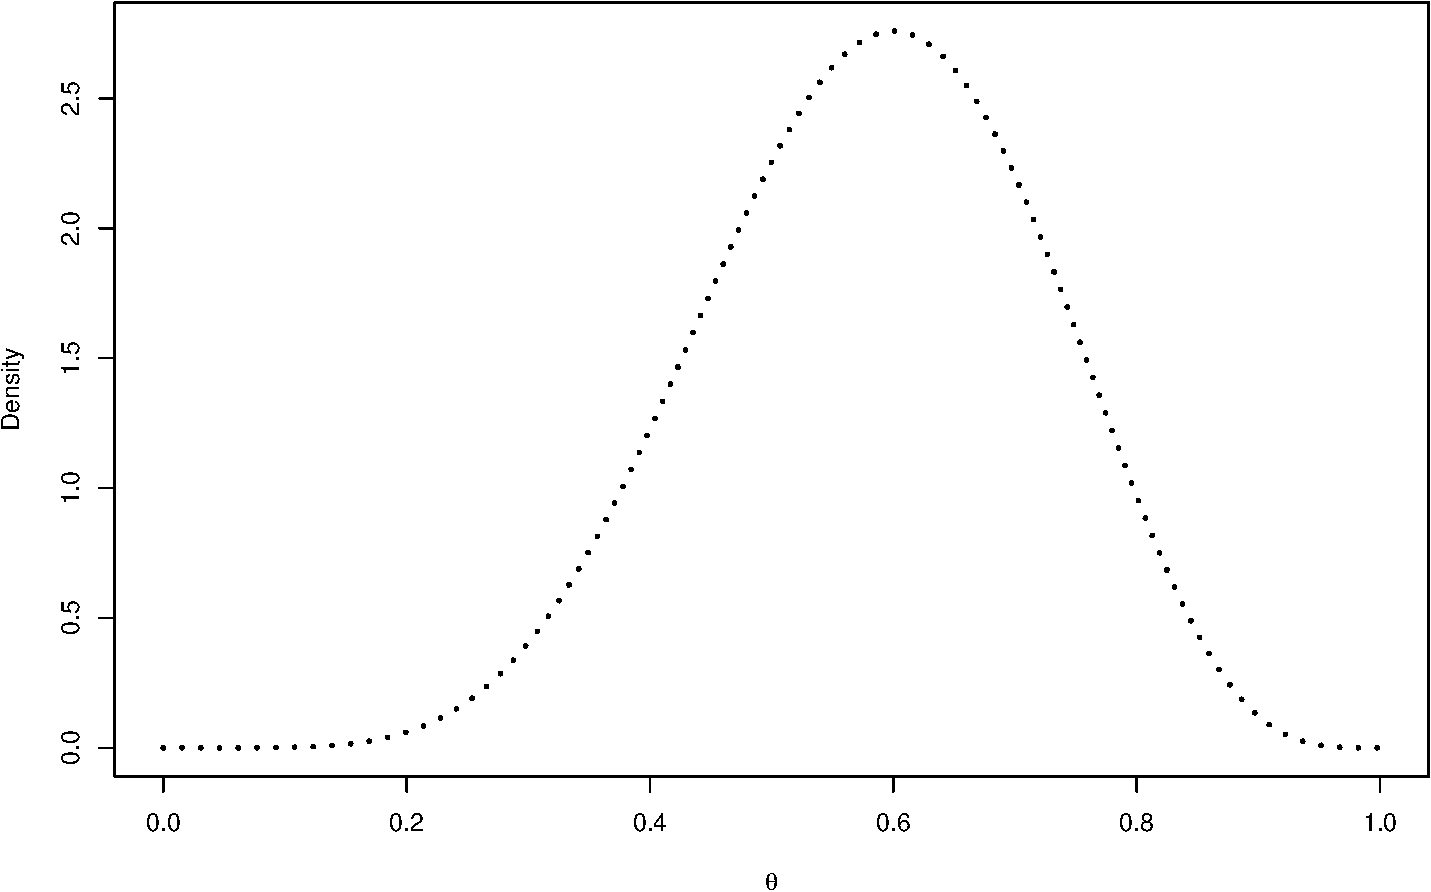
\includegraphics{01-intro-to-Bayes_files/figure-beamer/unnamed-chunk-2-1.pdf}

\end{frame}

\begin{frame}[fragile]{Prior}
\protect\hypertarget{prior}{}

\begin{Shaded}
\begin{Highlighting}[]
\KeywordTok{plot}\NormalTok{(th, prior, }\DataTypeTok{type=}\StringTok{'l'}\NormalTok{, }\DataTypeTok{ylab =} \StringTok{"Density"}\NormalTok{, }
     \DataTypeTok{lty =} \DecValTok{3}\NormalTok{, }\DataTypeTok{lwd =} \DecValTok{3}\NormalTok{, }\DataTypeTok{xlab =} \KeywordTok{expression}\NormalTok{(theta))}
\end{Highlighting}
\end{Shaded}

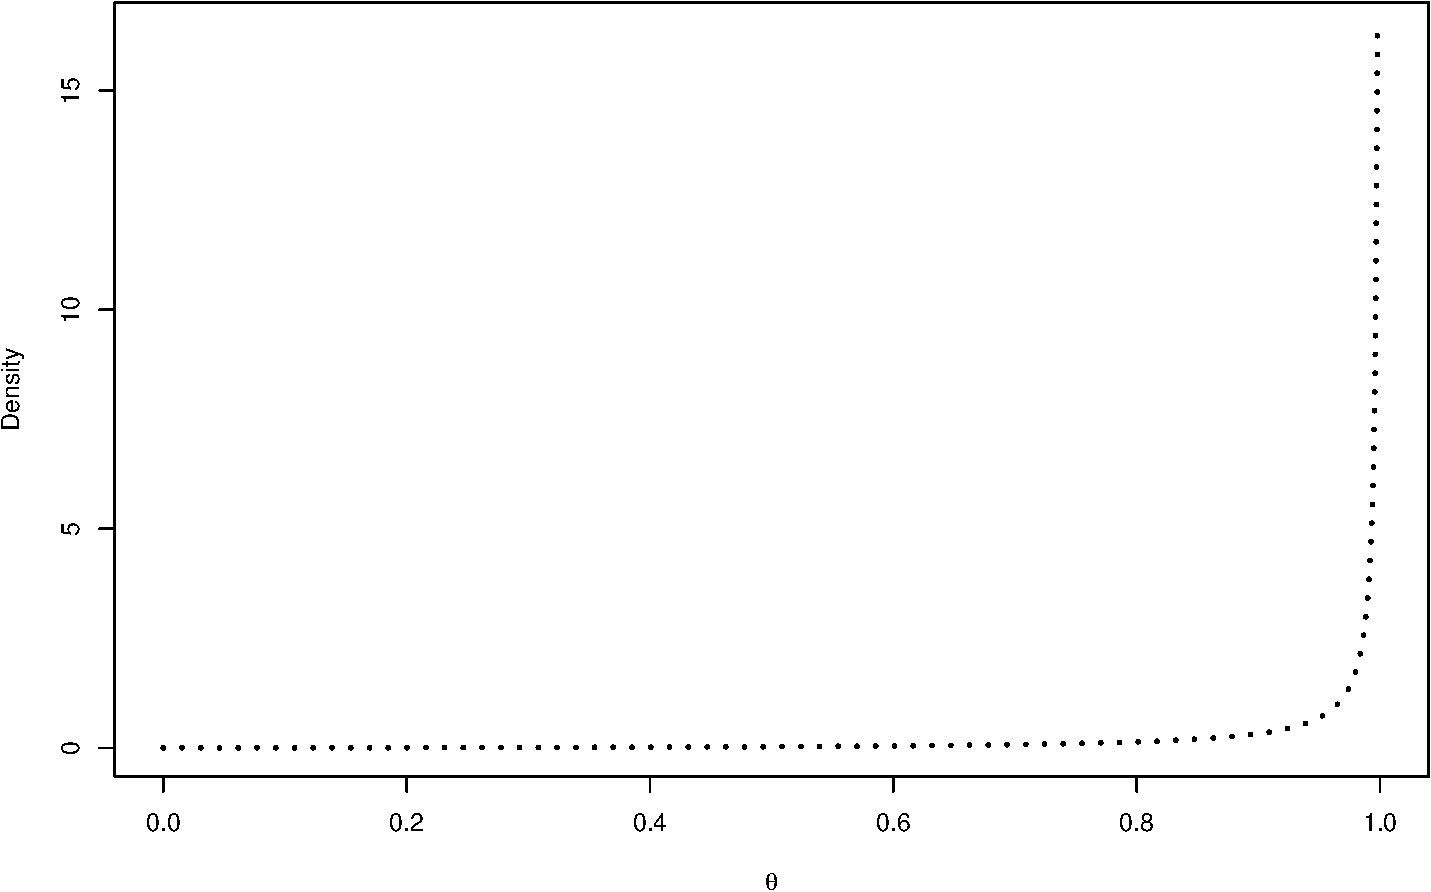
\includegraphics{01-intro-to-Bayes_files/figure-beamer/unnamed-chunk-3-1.pdf}

\end{frame}

\begin{frame}[fragile]{Posterior}
\protect\hypertarget{posterior}{}

\begin{Shaded}
\begin{Highlighting}[]
\KeywordTok{plot}\NormalTok{(th, post, }\DataTypeTok{type=}\StringTok{'l'}\NormalTok{, }\DataTypeTok{ylab =} \StringTok{"Density"}\NormalTok{, }
     \DataTypeTok{lty =} \DecValTok{3}\NormalTok{, }\DataTypeTok{lwd =} \DecValTok{3}\NormalTok{, }\DataTypeTok{xlab =} \KeywordTok{expression}\NormalTok{(theta))}
\end{Highlighting}
\end{Shaded}

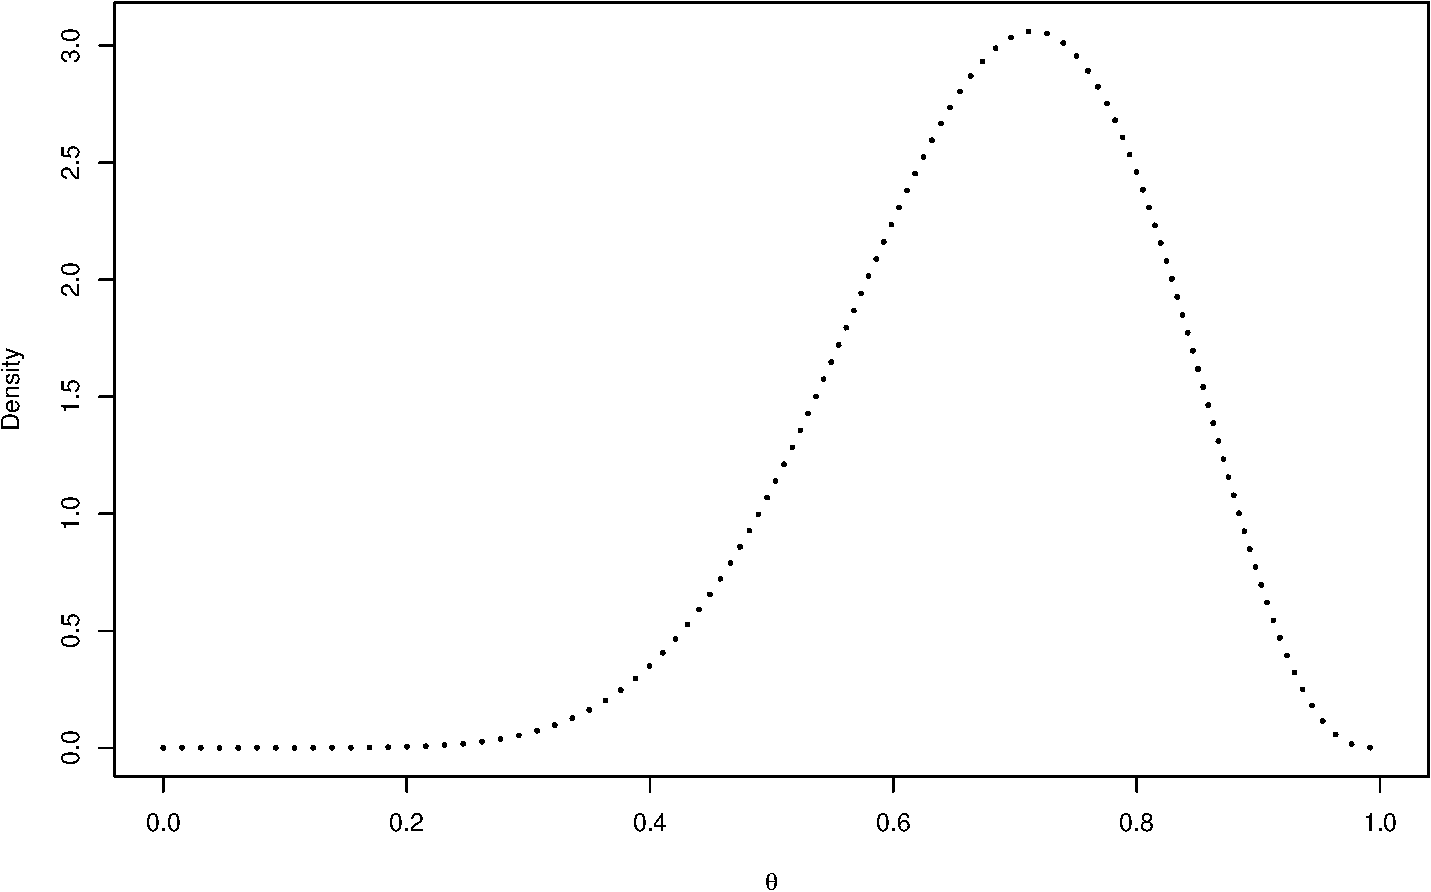
\includegraphics{01-intro-to-Bayes_files/figure-beamer/unnamed-chunk-4-1.pdf}

\end{frame}

\begin{frame}{Likelihood, Prior, and Posterior}
\protect\hypertarget{likelihood-prior-and-posterior}{}

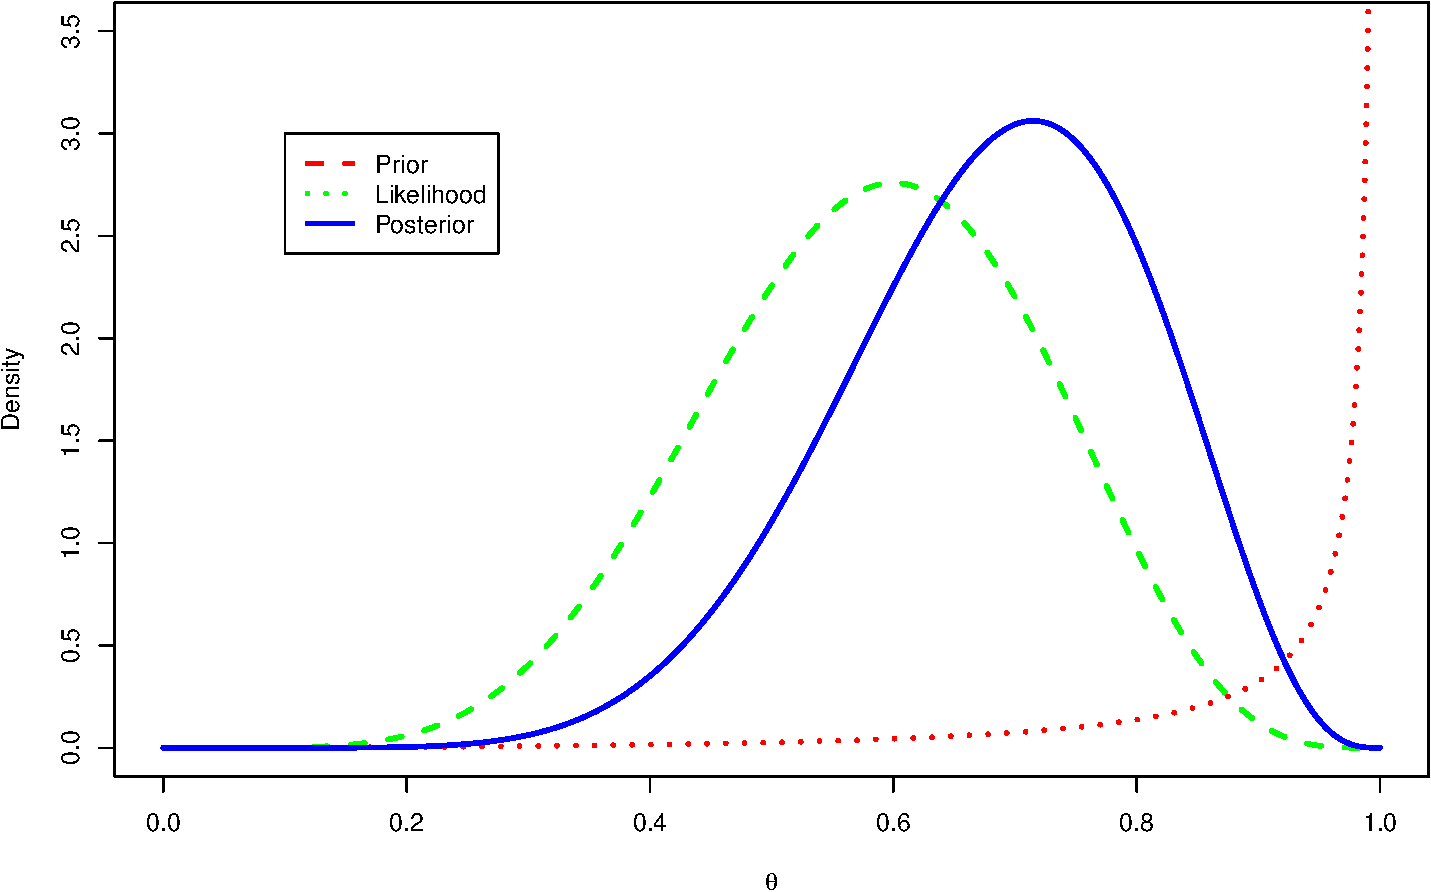
\includegraphics{01-intro-to-Bayes_files/figure-beamer/unnamed-chunk-5-1.pdf}

\end{frame}

\begin{frame}{Back to the Prior}
\protect\hypertarget{back-to-the-prior}{}

\begin{itemize}
\item
  We choose the prior here very arbitrarly due to very little
  information of ``subjective knowledge.''
\item
  Let's consider an example where we have more infomation and can set
  \(a,b\) from such subjective information.
\end{itemize}

\end{frame}

\begin{frame}{How Much Do You Sleep Example}
\protect\hypertarget{how-much-do-you-sleep-example}{}

We are interested in a population of American college students and the
proportion of the population that sleep at least eight hours a night,
which we denote by \(\theta.\)

\end{frame}

\begin{frame}{How Much Do You Sleep Example}
\protect\hypertarget{how-much-do-you-sleep-example-1}{}

\begin{itemize}

\item  \emph{The Gamecock}, at the USC printed an internet article ``College Students Don't Get Enough Sleep" (2004).  \begin{itemize}
\item Most students spend six hours sleeping each night. 
\end{itemize}
\item 2003: University of Notre Dame's paper, \emph{Fresh Writing}. 
\begin{itemize}
\item The article  reported took random sample of 100 students:
\item ``approximately 70\% reported to receiving only five to six hours of sleep on the weekdays, 
\item 28\% receiving seven to eight, 
\item and only 2\% receiving the healthy nine hours for teenagers."
\end{itemize}
\end{itemize}

\end{frame}

\begin{frame}{How Much Do You Sleep}
\protect\hypertarget{how-much-do-you-sleep}{}

\begin{itemize}
\item  Have a random sample of 27 students is taken from UF. 
\item 11 students record that they sleep at least eight hours each night. 
\item Based on this information, we are interested in estimating $\theta.$ 
\end{itemize}

\end{frame}

\begin{frame}{How Much Do You Sleep}
\protect\hypertarget{how-much-do-you-sleep-1}{}

\begin{itemize}
\item From USC and UND,  believe it's probably true that most college students get less than eight hours of sleep. 
\item Want our prior to assign most of the probability to values of $\theta < 0.5. $
\item From the information given, we decide that our best guess for $\theta$ is 0.3, although we think it is very possible that $\theta$ could be any value in $[0,0.5].$
\end{itemize}

\end{frame}

\begin{frame}{Our Model}
\protect\hypertarget{our-model}{}

Our model can be summarized by the Binomial-Beta distribution

\begin{align}
X|\theta &\sim \text{Binomial} (n, \theta) \\
\theta &\sim \text{Beta}(a,b) 
\end{align}

You can show that the posterior of
\[\theta \mid X \sim \text{Beta}(x+a,n-x+b)\]

\end{frame}

\begin{frame}{Choice of a,b for Beta Prior}
\protect\hypertarget{choice-of-ab-for-beta-prior}{}

\begin{itemize}
\item Given this information, we believe that the median of $\theta$ is $0.3$ and the $90$th percentile is 0.5. 
\item Knowing this allows us to estimate the unknown values of $a$ and $b$. 
\item How do we actually calculate $a$ and $b$?
\end{itemize}

\end{frame}

\begin{frame}{Choice of a,b for Beta Prior}
\protect\hypertarget{choice-of-ab-for-beta-prior-1}{}

We would need to solve the following equations:

\[\int_{0}^{0.3} \frac{\Gamma(a+b)}{\Gamma(a)\Gamma(b)}
\theta^{a-1}(1-\theta)^{b-1}\;d\theta = 0.5\]
\[\int_{0}^{0.5} \frac{\Gamma(a+b)}{\Gamma(a)\Gamma(b)}
\theta^{a-1}(1-\theta)^{b-1}\;d\theta = 0.9\]

In non-calculus language, this means the 0.5 quantile (50th
percentile)\textsubscript{=}0.3. The 0.9 quantile (90th percentile) =
0.5.

The equations are written as percentiles above!

\begin{itemize}
\item We can easily solve this numerically in \texttt{R} using a numerical solver \texttt{BBsolve} using the \texttt{BB} package. . 
\item The documentation for this package is not great, so beware.
\end{itemize}

\end{frame}

\begin{frame}[fragile]{How Much Do You Sleep}
\protect\hypertarget{how-much-do-you-sleep-2}{}

\begin{Shaded}
\begin{Highlighting}[]
\CommentTok{#load the BB package}
\KeywordTok{library}\NormalTok{(BB)}

\CommentTok{## using percentiles}
\NormalTok{myfn <-}\StringTok{ }\ControlFlowTok{function}\NormalTok{(shape)\{}
\NormalTok{    test <-}\StringTok{ }\KeywordTok{pbeta}\NormalTok{(}\DataTypeTok{q =} \KeywordTok{c}\NormalTok{(}\FloatTok{0.3}\NormalTok{, }\FloatTok{0.5}\NormalTok{), }\DataTypeTok{shape1 =}\NormalTok{ shape[}\DecValTok{1}\NormalTok{], }
     \DataTypeTok{shape2 =}\NormalTok{ shape[}\DecValTok{2}\NormalTok{]) }\OperatorTok{-}\StringTok{ }\KeywordTok{c}\NormalTok{(}\FloatTok{0.5}\NormalTok{, }\FloatTok{0.9}\NormalTok{)}
    \KeywordTok{return}\NormalTok{(test)}
\NormalTok{    \}}
\KeywordTok{BBsolve}\NormalTok{(}\KeywordTok{c}\NormalTok{(}\DecValTok{1}\NormalTok{,}\DecValTok{1}\NormalTok{), myfn)}
\end{Highlighting}
\end{Shaded}

\begin{verbatim}
##   Successful convergence.
\end{verbatim}

\begin{verbatim}
## $par
## [1] 3.263743 7.185121
## 
## $residual
## [1] 5.905161e-08
## 
## $fn.reduction
## [1] 3.521457e-05
## 
## $feval
## [1] 115
## 
## $iter
## [1] 20
## 
## $convergence
## [1] 0
## 
## $message
## [1] "Successful convergence"
## 
## $cpar
## method      M     NM 
##      2     50      1
\end{verbatim}

\begin{Shaded}
\begin{Highlighting}[]
\CommentTok{## using quantiles}
\NormalTok{fn =}\StringTok{ }\ControlFlowTok{function}\NormalTok{(x)\{}\KeywordTok{qbeta}\NormalTok{(}\KeywordTok{c}\NormalTok{(}\FloatTok{0.5}\NormalTok{,}\FloatTok{0.9}\NormalTok{),x[}\DecValTok{1}\NormalTok{],x[}\DecValTok{2}\NormalTok{])}\OperatorTok{-}\KeywordTok{c}\NormalTok{(}\FloatTok{0.3}\NormalTok{,}\FloatTok{0.5}\NormalTok{)\}}
\NormalTok{estimated <-}\StringTok{ }\KeywordTok{BBsolve}\NormalTok{(}\KeywordTok{c}\NormalTok{(}\DecValTok{1}\NormalTok{,}\DecValTok{1}\NormalTok{),fn)}
\end{Highlighting}
\end{Shaded}

\begin{verbatim}
##   Successful convergence.
\end{verbatim}

\end{frame}

\begin{frame}{How Much Do You Sleep}
\protect\hypertarget{how-much-do-you-sleep-3}{}

Using our calculations from the Beta-Binomial our model is
\begin{align*}
X \mid \theta &\sim \textrm{Binomial}(27,\theta)\\
\theta &\sim \textrm{Beta}(3.3,7.2)\\
\theta \mid x &\sim \textrm{Beta}(x+3.3,27-x+7.2)\\
\theta \mid 11 &\sim \textrm{Beta}(14.3,23.2)\\
\end{align*}

\end{frame}

\begin{frame}[fragile]{How Much Do You Sleep}
\protect\hypertarget{how-much-do-you-sleep-4}{}

\begin{Shaded}
\begin{Highlighting}[]
\NormalTok{th =}\StringTok{ }\KeywordTok{seq}\NormalTok{(}\DecValTok{0}\NormalTok{,}\DecValTok{1}\NormalTok{,}\DataTypeTok{length=}\DecValTok{500}\NormalTok{)}
\NormalTok{a =}\StringTok{ }\NormalTok{estimated}\OperatorTok{$}\NormalTok{par[}\DecValTok{1}\NormalTok{]}
\NormalTok{b =}\StringTok{ }\NormalTok{estimated}\OperatorTok{$}\NormalTok{par[}\DecValTok{2}\NormalTok{]}
\NormalTok{n =}\StringTok{ }\DecValTok{27}
\NormalTok{x =}\StringTok{ }\DecValTok{11}
\NormalTok{prior =}\StringTok{ }\KeywordTok{dbeta}\NormalTok{(th,a,b)}
\NormalTok{like =}\StringTok{ }\KeywordTok{dbeta}\NormalTok{(th,x}\OperatorTok{+}\DecValTok{1}\NormalTok{,n}\OperatorTok{-}\NormalTok{x}\OperatorTok{+}\DecValTok{1}\NormalTok{)}
\NormalTok{post =}\StringTok{ }\KeywordTok{dbeta}\NormalTok{(th,x}\OperatorTok{+}\NormalTok{a,n}\OperatorTok{-}\NormalTok{x}\OperatorTok{+}\NormalTok{b)}
\KeywordTok{plot}\NormalTok{(th,post,}\DataTypeTok{type=}\StringTok{"l"}\NormalTok{,}\DataTypeTok{ylab=}\StringTok{"Density"}\NormalTok{,}\DataTypeTok{lty=}\DecValTok{2}\NormalTok{,}\DataTypeTok{lwd=}\DecValTok{3}\NormalTok{,}
\DataTypeTok{xlab =} \KeywordTok{expression}\NormalTok{(theta))}
\KeywordTok{lines}\NormalTok{(th,like,}\DataTypeTok{lty=}\DecValTok{1}\NormalTok{,}\DataTypeTok{lwd=}\DecValTok{3}\NormalTok{)}
\KeywordTok{lines}\NormalTok{(th,prior,}\DataTypeTok{lty=}\DecValTok{3}\NormalTok{,}\DataTypeTok{lwd=}\DecValTok{3}\NormalTok{)}
\KeywordTok{legend}\NormalTok{(}\FloatTok{0.7}\NormalTok{,}\DecValTok{4}\NormalTok{,}\KeywordTok{c}\NormalTok{(}\StringTok{"Prior"}\NormalTok{,}\StringTok{"Likelihood"}\NormalTok{,}\StringTok{"Posterior"}\NormalTok{),}
\DataTypeTok{lty=}\KeywordTok{c}\NormalTok{(}\DecValTok{3}\NormalTok{,}\DecValTok{1}\NormalTok{,}\DecValTok{2}\NormalTok{),}\DataTypeTok{lwd=}\KeywordTok{c}\NormalTok{(}\DecValTok{3}\NormalTok{,}\DecValTok{3}\NormalTok{,}\DecValTok{3}\NormalTok{))}
\end{Highlighting}
\end{Shaded}

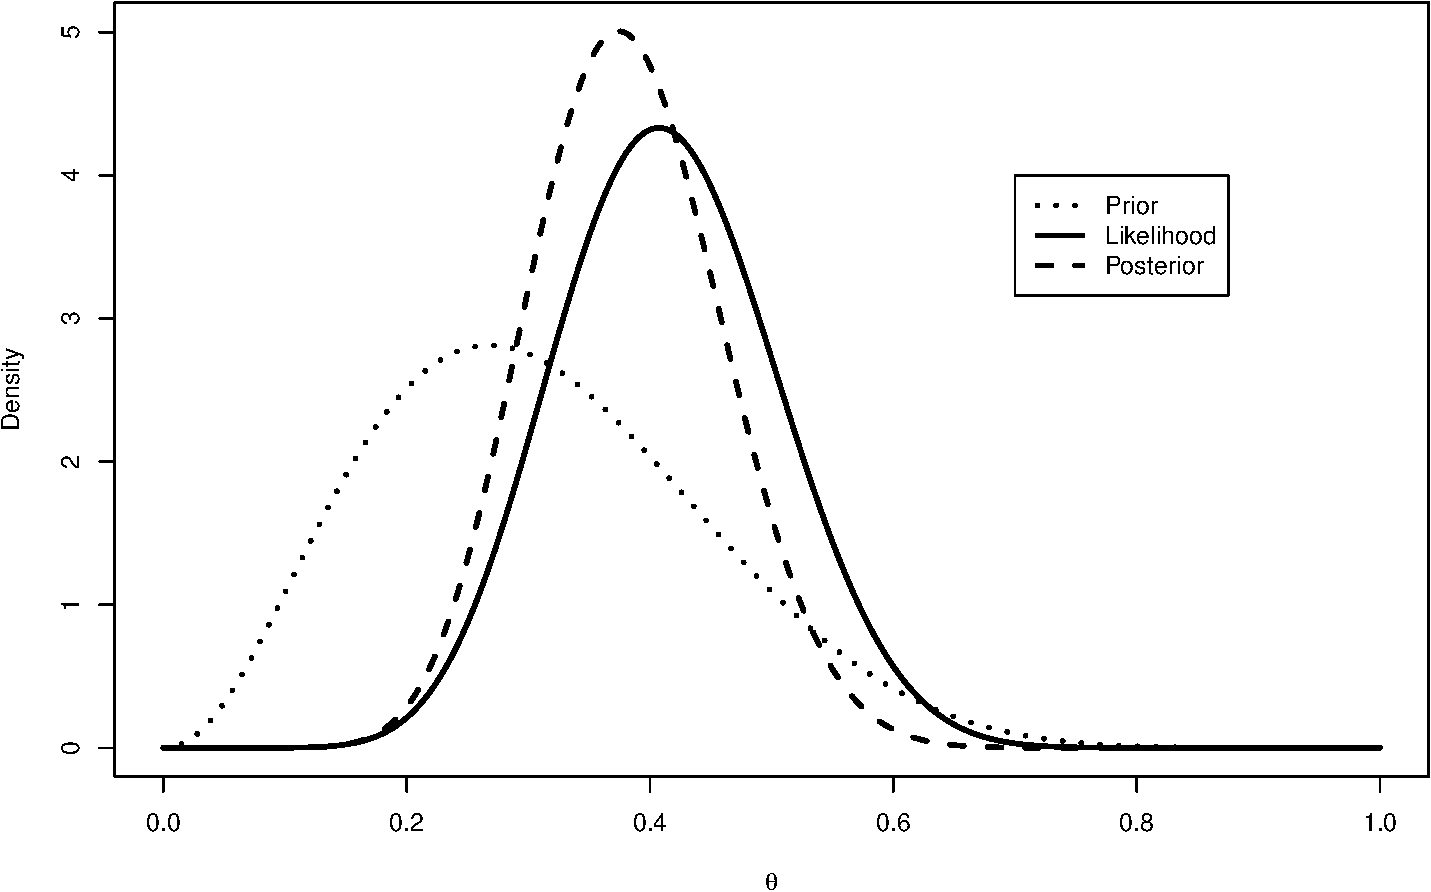
\includegraphics{01-intro-to-Bayes_files/figure-beamer/unnamed-chunk-7-1.pdf}

\end{frame}

\begin{frame}{How Much Do You Sleep}
\protect\hypertarget{how-much-do-you-sleep-5}{}

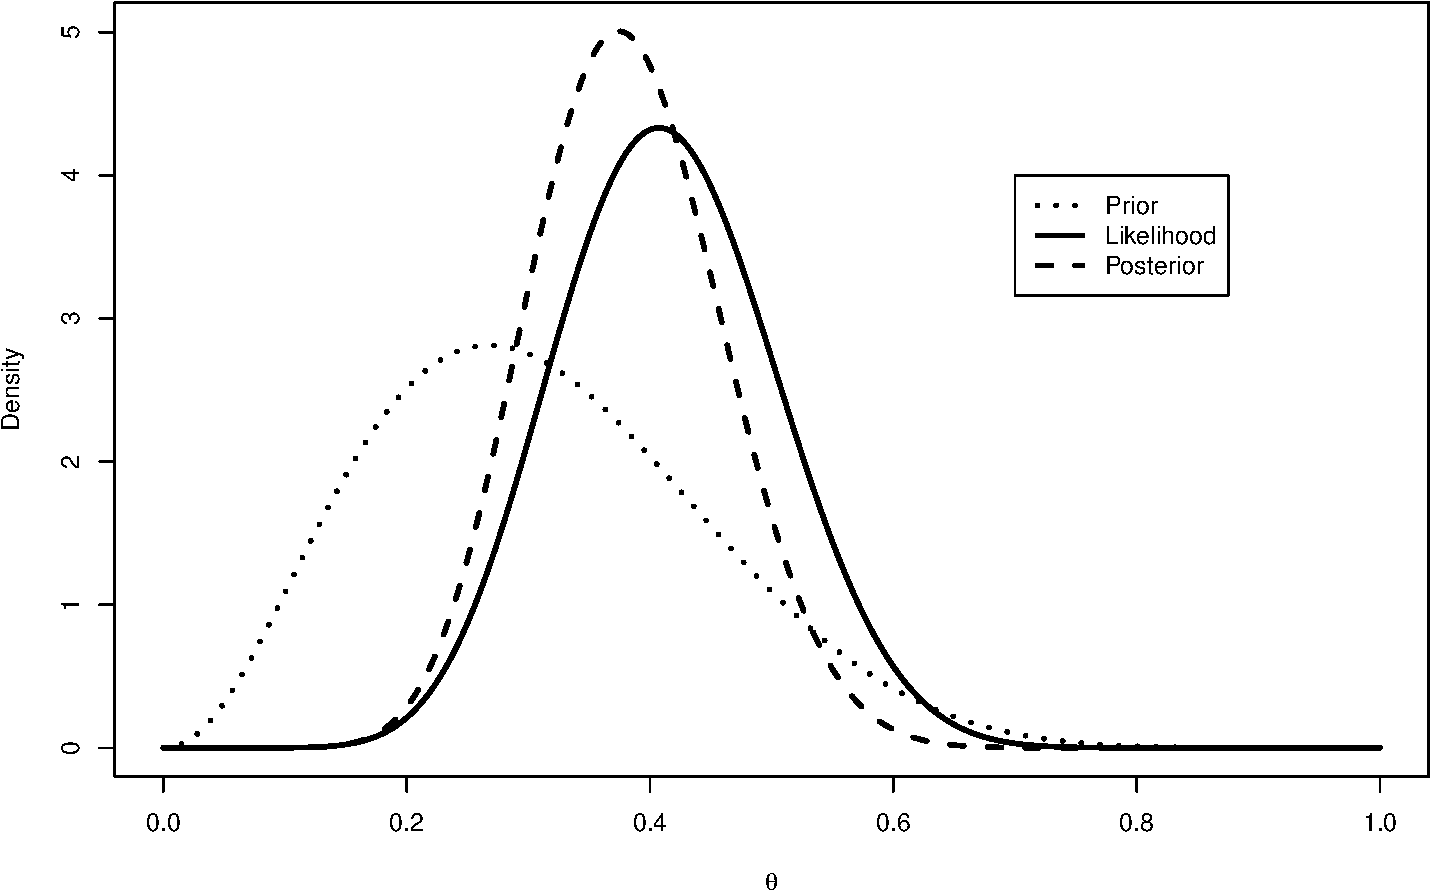
\includegraphics{01-intro-to-Bayes_files/figure-beamer/unnamed-chunk-8-1.pdf}

\end{frame}

\begin{frame}{Cast of characters}
\protect\hypertarget{cast-of-characters}{}

\begin{itemize}
\tightlist
\item
  Observed data: \(x\)
\item
  Note this could consist of many data points, e.g.,
  \(x = x_{1:n}=(x_1,\dotsc,x_n)\).
\end{itemize}

\begin{center}
\begin{tabular}{ l l }
likelihood & $p(x|\theta)$  \\
prior & $p(\theta)$ \\
posterior & $p(\theta|x)$ \\
marginal likelihood & $p(x)$ \\
posterior predictive & $p(x_{n+1}|x_{1:n})$ \\
loss function & $\ell(s,a)$ \\
posterior expected loss & $\rho(a,x)$ \\
risk / frequentist risk & $R(\theta,\delta)$ \\
integrated risk & $r(\delta)$
\end{tabular}
\end{center}

\end{frame}

\begin{frame}{Marginal likelihood}
\protect\hypertarget{marginal-likelihood}{}

The \textbf{marginal likelihood} is
\[ p(x) = \int p(x|\theta) p(\theta) \,d\theta \]

\begin{itemize}
\tightlist
\item
  What is the marginal likelihood for the Bernoulli-Beta?
\end{itemize}

\end{frame}

\begin{frame}{Example: Back to the Bernoulli-Beta}
\protect\hypertarget{example-back-to-the-bernoulli-beta}{}

Suppose \[\; \theta\sim Beta(a,b)\] and
\[X_1,\dotsc,X_n\mid \theta \stackrel{iid}{\sim} Bernoulli(\theta)\]

\end{frame}

\begin{frame}{Example: Back to the Bernoulli-Beta}
\protect\hypertarget{example-back-to-the-bernoulli-beta-1}{}

Then the marginal likelihood is \[
\begin{aligned}
&p(x_{1:n}) \\
&= \int p(x_{1:n}|\theta) p(\theta) \,d\theta\\
& = \int_0^1\theta^{\sum x_i}(1-\theta)^{n-\sum x_i}\frac{1}{B(a,b)}\theta^{a-1}(1-\theta)^{b-1} d\theta\\
& = \frac{1}{B(a,b)}\int_0^1\theta^{\sum x_i+a-1}(1-\theta)^{n-\sum x_i+b-1} 
d\theta\\
& = \frac{\textcolor{red}{B\big(a +\sum x_i,\, b + n-\sum x_i\big)}}{B(a,b)}\int_0^1 \frac{\theta^{\sum x_i+a-1}(1-\theta)^{n-\sum x_i+b-1}}{\textcolor{red}{B\big(a +\sum x_i,\, b + n-\sum x_i\big)}}
d\theta\\
& =\frac{B\big(a +\sum x_i,\, b + n-\sum x_i\big)}{B(a,b)},
\end{aligned}
\] by the integral definition of the Beta function.

\end{frame}

\begin{frame}{Posterior predictive distribution}
\protect\hypertarget{posterior-predictive-distribution}{}

Let \(a_n = a +\sum x_i\) and \(b_n = b + n-\sum x_i.\)

Recall that the posterior distribution is
\(p(\theta|x_{1:n}) = \Beta(\theta|a_n,b_n).\)

Let's derive the posterior preditive distribution.

\end{frame}

\begin{frame}{Posterior predictive distribution}
\protect\hypertarget{posterior-predictive-distribution-1}{}

\begin{itemize}
\tightlist
\item
  We may wish to predict a new data point \(x_{n+1}\)
\item
  \textcolor{red}{Assumption 1}: Assume that \(x_{1:(n+1)}\) are
  independent given \(\theta\)
\end{itemize}

\[
\begin{aligned}
p(x_{n+1}|x_{1:n}) &= \int p(x_{n+1},\theta|x_{1:n})\,d\theta\\
& \int \frac{p(x_{n+1},\theta, x_{1:n})}{p(x_{1:n})}\,d\theta \quad (\text{Conditional probability})\\
& \int \frac{p(x_{n+1}|\theta,x_{1:n})p(\theta|x_{1:n})p(x_{1:n})}{p(x_{1:n})}\,d\theta \quad (\text{Product rule})\\
&= \int p(x_{n+1}|\theta,x_{1:n}) p(\theta|x_{1:n})\,d\theta \\
& = \int p(x_{n+1}|\theta) p(\theta|x_{1:n})\,d\theta \quad \text{By Assumption 1.}
\end{aligned}
\]

\end{frame}

\begin{frame}{Posterior predictive distribution}
\protect\hypertarget{posterior-predictive-distribution-2}{}

The posterior predictive can be derived to be \[
\begin{aligned}
\Pr(X_{n+1} = 1\mid x_{1:n}) 
&= \int \Pr(X_{n+1} = 1\mid \theta) p(\theta|x_{1:n}) d\theta\\
& =\int \theta\,\Beta(\theta|a_n,b_n) d\theta \\
& =\frac{a_n}{a_n + b_n}  \quad (\text{Mean of Beta distribution}).
\end{aligned}
\]

Similarly, \[
\begin{aligned}
\Pr(X_{n+1} = 0 \mid x_{1:n}) & = 1- \Pr(X_{n+1} = 1 \mid x_{1:n}) = \frac{b_n}{a_n + b_n}.
\end{aligned}
\]

\end{frame}

\begin{frame}{Posterior predictive distribution (continued)}
\protect\hypertarget{posterior-predictive-distribution-continued}{}

This implies that

\[p(x_{n+1}|x_{1:n}) =
\begin{cases} 
 \frac{a_n}{a_n + b_n} & \mbox{if } x_{n+1} = 1  \\
\frac{b_n}{a_n + b_n} & \mbox{if } x_{n+1} = 0
\end{cases}
\]

Hence, the posterior predictive p.m.f. is

\[
\begin{aligned}
p(x_{n+1}|x_{1:n}) & = \frac{a_n^{x_{n+1}} b_n^{1-x_{n+1}}}{a_n + b_n}\I(x_{n+1}\in\{0,1\}).
\end{aligned}
\]

\end{frame}

\begin{frame}{Overall Summary}
\protect\hypertarget{overall-summary}{}

\begin{itemize}
\tightlist
\item
  We covered the ``cast of characters'' needed to work with Bayesian
  models
\item
  These include the likelihood, prior, posterior, marginal likelihood,
  and posterior predictive distribution
\item
  We derived Bayes' Theorem
\item
  Bernoulli-Beta
\item
  Conjugacy
\end{itemize}

\end{frame}

\begin{frame}{Background Knowledge}
\protect\hypertarget{background-knowledge}{}

\begin{itemize}
\tightlist
\item
  Familiar with Discrete and Continuous Distributions
\item
  Can calculate expectations and variances
\item
  Change of variables
\item
  Mean squared error
\item
  Sufficiency
\item
  Confident calculating the likelihood and log-likelihood
\item
  Confident in working with partial derivatives
\item
  Familiar maximizing or minimizing functions (and proving they are
  global max/min)
\end{itemize}

\end{frame}

\begin{frame}{Detailed Summary for Exam}
\protect\hypertarget{detailed-summary-for-exam}{}

\begin{itemize}
\tightlist
\item
  Bayes Theorem
\item
  Likelihood
\item
  Prior
\item
  Posterior derivation
\item
  Marginal likelihood
\item
  Posterior predictive distribution
\item
  Conjugacy
\item
  Proportionality
\item
  Understanding when models are appropriate for data given to you (Ex:
  Approval ratings for Obama)
\item
  What is an informative prior
\item
  What is a non-informative prior
\item
  Proper posterior
\item
  How do you incorporate a pilot study into your posterior analysis (Ex:
  See sleep study)
\end{itemize}

\end{frame}

\begin{frame}{Exercise}
\protect\hypertarget{exercise}{}

We write \(X\sim\Poisson(\theta)\) if \(X\) has the Poisson distribution
with rate \(\theta>0\), that is, its p.m.f.~is
\[ p(x|\theta) = \Poisson(x|\theta)= e^{-\theta} \theta^x / x!\] for
\(x\in\{0,1,2,\dotsc\}\) (and is \(0\) otherwise). Suppose
\(X_1,\dotsc,X_n \stackrel{iid}{\sim} \Poisson(\theta)\) given
\(\theta\), and your prior is
\[ p(\theta) =\Ga(\theta|a,b) =\frac{b^a}{\Gamma(a)} \theta^{a-1} e^{-b\theta}\I(\theta>0) .\]
What is the posterior distribution on \(\theta\)?

\end{frame}

\begin{frame}{Solution}
\protect\hypertarget{solution}{}

Since the data is independent given \(\theta\), the likelihood factors
and we get \begin{align*}
p(x_{1:n}|\theta) & = \prod_{i = 1}^n p(x_i|\theta) \\
& = \prod_{i = 1}^n e^{-\theta} \theta^{x_i} / x_i! \\
& \underset{\theta}{\propto} e^{-n\theta} \theta^{\sum x_i}.
\end{align*}

\end{frame}

\begin{frame}{Solution}
\protect\hypertarget{solution-1}{}

Thus, using Bayes' theorem, \begin{align*}
p(\theta|x_{1:n}) &\propto p(x_{1:n}|\theta) p(\theta) \\
& \propto e^{-n\theta} \theta^{\sum x_i} \theta^{a-1} e^{-b\theta}\I(\theta>0) \\
& \propto e^{-(b+n)\theta} \theta^{a+\sum x_i-1}\I(\theta>0) \\
& \propto \Ga\big(\theta\mid a+\textstyle\sum x_i,\,b+n\big).
\end{align*} Therefore, since the posterior density must integrate to
\(1\), we have
\[p(\theta|x_{1:n}) =\Ga\big(\theta\mid a+\textstyle\sum x_i,\,b+n\big).\]

\end{frame}

\end{document}
